\documentclass[11pt,a4paper]{article}
\usepackage[T1]{fontenc}\usepackage[utf8]{inputenc}
\usepackage{lmodern,microtype,amsmath,amssymb,amsthm,mathtools}
\usepackage{booktabs,longtable,array,enumitem,xcolor,geometry,fancyhdr,hyperref,graphicx}
\geometry{margin=22mm}
\hypersetup{colorlinks=true,linkcolor=blue!55!black,urlcolor=blue,citecolor=blue!55!black,
 pdftitle={FIN ST2082--ST2171: Equivariant Second-Differential Classification, Hodge-Spectral No-Go and the Three-Point Source Frontier},
 pdfauthor={Krzysztof Żuchowski}}
\pagestyle{fancy}\fancyhf{}\fancyhead[L]{FIN ST2082--ST2171}\fancyhead[R]{Release 11.07}\fancyfoot[C]{\thepage}\setlength{\headheight}{14pt}
\newtheorem{theorem}{Theorem}\newcommand{\status}[1]{\textsf{[#1]}}

\begin{document}
\begin{titlepage}\centering\vspace*{14mm}
{\Huge\bfseries FIN ST2082--ST2171\par}\vspace{4mm}
{\LARGE Equivariant Second-Differential Classification,\par}\vspace{2mm}
{\LARGE Hodge-Spectral No-Go and the Three-Point Source Frontier\par}\vspace{12mm}
{\Large Krzysztof \.Zuchowski\par}
{\normalsize Independent Researcher --- Fractal Information Theory Project\par}
{\normalsize ORCID: 0009-0002-0909-3613\par}\vspace{9mm}
{\large Six adaptive research rounds --- 90 programmes\par}
{\large Release 11.07 --- 1 September 2026\par}
\vfill
\begin{minipage}{.87\textwidth}\small
This report executes the equivariant-second-differential problem selected in
Release 11.06.  It computes the exact $D_{12}$ representation-theoretic
dimension, imposes locality, integral cellular incidence and refinement
intertwining, then audits positivity, Hodge rescaling, spectra and continuum
claims.  The resulting no-go identifies the missing information type as an
intrinsic ternary/2-form source rather than another pairwise-kernel function.
\end{minipage}\vfill
{\small English mathematical and critical research report.}
\end{titlepage}

\begin{abstract}
ST2082--ST2171 classify possible second differentials
$d_1:C^1\to C^2$ for the strict FIN carrier.  On the full oriented simplex,
exact $D_{12}$ character theory gives
\[
\dim\operatorname{Hom}_{D_{12}}(C^1,C^2)=615.
\]
Since the gradient image is isomorphic to $C^0/\mathbf1$, the maps satisfying
$d_1d_0=0$ form
\[
\operatorname{Hom}_{D_{12}}(C^1/\operatorname{im}d_0,C^2)
\]
of exact dimension
\[
\boxed{517}.
\]
Thus equivariance and the chain condition alone are radically nonunique.

Boundary locality collapses the problem.  On one oriented triangle, a local
row $a x_{ij}+b x_{jk}+c x_{ik}$ annihilates all gradients if and only if it is
proportional to the standard oriented boundary $(1,1,-1)$.  $D_{12}$
equivariance leaves one scalar for each of the twelve triangle orbits, producing
a 12-dimensional family.  Requiring primitive integral cellular incidence
restricts every nonzero orbit scalar to $\pm1$, and face orientation absorbs
the signs.  Therefore standard $d_1$ is combinatorially unique only after a
face complex and integral cell basis have already been chosen.

Refinement does not supply the missing choice.  The cochain intertwiner fixes
the coefficients of lifted triangles but every product-square row annihilates
pulled-back base edge cochains.  Six vertical square-orbit coefficients remain
at level 24 and at least thirteen after level 48.  Primitive cellular incidence
again yields an associative standard coboundary, but only relative to the
chosen product-cell history.

The distinction between differential normalization and Hodge measure is
essential.  Writing a row scale $c_f$ and positive face weight $m_f$, the
curvature operator depends only on
\[
h_f=m_fc_f^2.
\]
Row/Hodge inverse rescaling is an exact gauge of description.  After quotienting
it, physical positive quadratic forms still form an $(\mathbb R_+)^{12}$ orbit
cone.  All positive orbit scales preserve the same cohomology kernel, so
topology does not select them.

For the unweighted full simplex an exact identity holds:
\[
L_1=d_0d_0^*+d_1^*d_1=12I_{66}.
\]
The standard one-form spectrum is completely flat.  Positive orbit Hodge
weights split it into 33 distinct rounded eigenvalues in an explicit witness
without changing $H^1$.  Hence no nonzero gauge spectral prediction is invariant
over the admissible Hodge cone.  Spectral actions and effective dimensions add
further cutoff/scale dependence.

The classification can be summarized as
\[
517\xrightarrow{\rm locality}12
\xrightarrow{\rm primitive\ integral\ cells}1,
\]
where the final arrow is conditional on exactly the face/cell structure that
strict FIN has not sourced.  Pairwise kernel and 0-form Dirichlet data contain
no independent three-point face observable.  The highest-value next theorem is
therefore to derive or refute an intrinsic strict ternary cumulant/associator or
cycle observable with a $D_{12}$ transformation law, nonzero orbit witness and
refinement coherence.  Without such a new information type, unique gauge
geometry cannot emerge from the current pairwise data without assumption.
\end{abstract}

\tableofcontents\newpage

\section{Round I: ST2082--ST2096 --- exact character classification}

Let $C^0,C^1,C^2$ be oriented vertex, edge and triangle cochain spaces of the
full 11-simplex on twelve vertices.  Their dimensions are
\[
12,\qquad 66,\qquad 220.
\]
The dihedral group acts with orientation signs.  For a group element $g$, the
character $\chi_k(g)$ is the signed count of oriented $(k+1)$-vertex subsets
fixed as sets by $g$.  Exact enumeration over all 24 group elements gives the
oriented character table used in this report.

The dimension of equivariant maps is the character inner product:
\[
\dim\operatorname{Hom}_{D_{12}}(C^1,C^2)
=\frac1{24}\sum_g\chi_1(g)\chi_2(g)=615.
\]
For the connected complete graph,
\[
\operatorname{im}d_0\cong C^0/\mathbf1,
\]
with character $\chi_0-1$.  Therefore the edge quotient has character
$\chi_1-\chi_0+1$ and dimension 55.  Maschke splitting gives
\[
\dim\{T:C^1\to C^2\mid T\text{ equivariant},\ Td_0=0\}
=\frac1{24}\sum_g(\chi_1-\chi_0+1)\chi_2=517.
\]

\begin{theorem}[equivariant chain-map no-go]
$D_{12}$ equivariance and $d_1d_0=0$ leave a 517-dimensional real solution
space on the full triangle representation.  They cannot determine a unique
second differential.
\end{theorem}

Reflection orientation signs are essential; an unoriented fixed-set census
would compute a different and inappropriate representation.

\section{Round II: ST2097--ST2111 --- boundary locality}

For one oriented triangle $i<j<k$, take
\[
(Tx)_{ijk}=a x_{ij}+b x_{jk}+c x_{ik}.
\]
On a gradient $x_{ij}=f_j-f_i$, exact symbolic coefficient matching gives
\[
(a,b,c)=t(1,1,-1).
\]
Thus a boundary-local row satisfying $Td_0=0$ is one-dimensional.  Equivariance
makes $t$ constant on each of the twelve triangle orbits, so locality reduces
the 517-dimensional space to twelve dimensions.

Setting all twelve scales to one gives the standard simplicial coboundary.
If every present face row must be a primitive integral cellular boundary, its
scale is $\pm1$.  Reversing the face orientation absorbs the sign.  Hence:

\begin{theorem}[conditional cellular uniqueness]
For a fixed oriented face complex with primitive integral incidence, the
boundary-local second differential is unique up to face orientation.
\end{theorem}

This does not select the face complex.  Full $S_{12}$ symmetry would make all
triangles one orbit, but it does not preserve the weighted strict operator.
Functions of strict edge weights can assign twelve distinct natural scales.

Nonzero row rescaling leaves $\ker d_1$ unchanged, so $H^1$ cannot select row
normalizations.

\section{Round III: ST2112--ST2126 --- refinement intertwiners}

Let $R_1$ pull a base edge cochain to identical horizontal copies and set
vertical edges to zero.  Let $R_2$ duplicate base face cochains and set product
squares to zero.  The refinement condition is
\[
R_2d_{1,12}=d_{1,24}R_1.
\]
It fixes each lifted triangle coefficient to the corresponding base-orbit
coefficient.  Every square boundary evaluates to zero on $R_1C^1$, so square
row coefficients are absent from the equation.  Six square-orbit coefficients
remain at level 24.

At the next binary refinement, all old coefficients are inherited while at
least seven new vertical edge-type coefficients appear.  The two-level vertical
moduli space has dimension at least 13 without primitive integrality.

If a product cell complex is chosen and primitive integral incidence imposed,
all rows become standard $\pm1$ cellular boundaries.  The resulting coboundary
is associative and satisfies $d_1d_0=0$ at every level.  This is a conditional
positive construction relative to the cell/refinement history, not a strict
selection.

\section{Round IV: ST2127--ST2141 --- Hodge and positivity}

There are two equivalent first-order conventions:
\begin{align*}
A&=d_0^*M_1d_0,\qquad M_1=\operatorname{diag}(w_e),\\
A&=(Rd_0)^*(Rd_0),\qquad R=\operatorname{diag}(\sqrt{w_e}).
\end{align*}
In the weighted-differential convention the compatible second differential is
\[
d_{1,w}=d_1R^{-1},
\]
so $d_{1,w}Rd_0=0$.  Weighting $d_0$ without compensating $d_1$ would violate
the chain condition.

For a face metric $M_2>0$, the curvature quadratic operator is
\[
Q_1=d_1^*M_2d_1\ge0.
\]
If face row $f$ is scaled by $c_f$ and its metric weight by $m_f$, the operator
depends only on
\[
h_f=m_fc_f^2.
\]
The transformation
\[
c_f\mapsto a_fc_f,\qquad m_f\mapsto a_f^{-2}m_f
\]
is an exact descriptive redundancy.  Quotienting it leaves one positive
quadratic coefficient per triangle orbit:
\[
h\in(\mathbb R_+)^{12}.
\]

Every strictly positive orbit choice has the same $d_1$ kernel of dimension 11
on edge cochains.  Topology fixes zero modes but not positive eigenvalues.

\section{Round V: ST2142--ST2156 --- spectral no-go}

For the unweighted complete simplex, exact matrix multiplication gives
\[
d_0d_0^*+d_1^*d_1=12I_{66}.
\]
All one-form Hodge modes have eigenvalue 12.  This fully symmetric choice has no
nontrivial dispersion structure.

Assigning different positive scales to the twelve $D_{12}$ triangle orbits
preserves $H^1=0$ but splits the one-form spectrum.  An explicit deterministic
choice produces 33 distinct rounded eigenvalues ranging from approximately 12
to 43.21.  Continuous changes of the Hodge cone continuously tune these values.

Consequently:
\begin{itemize}
\item cohomology controls only zero-mode dimensions after a complex is chosen;
\item positive gauge stiffness/mass scales remain free;
\item $\operatorname{Tr}f(L_1/\Lambda^2)$ depends on twelve Hodge parameters,
      the cutoff function and scale;
\item one-form heat traces and effective dimensions are measure dependent;
\item refinement flag zero modes can be removed with product squares only by
      introducing new vertical spectral parameters;
\item no Lorentz signature, wavevector locality or Maxwell normalization is
      produced.
\end{itemize}

\begin{theorem}[Hodge-spectral prediction no-go]
No nonzero one-form spectral prediction is invariant over the currently
admissible positive $D_{12}$-natural Hodge cone.  Integral incidence and fixed
cohomology do not select gauge dynamics.
\end{theorem}

\section{Round VI: ST2157--ST2171 --- final frontier}

The exact reduction ladder is
\[
\boxed{517\xrightarrow{\rm boundary\ locality}12
\xrightarrow{\rm primitive\ integral\ cells}1.}
\]
The final one-dimensional result is conditional on a chosen cell complex and
integral cellular basis.  Refinement adds unconstrained vertical coefficients,
and Hodge quotienting leaves twelve positive physical quadratic parameters at
the base level.

\begin{longtable}{@{}p{.37\textwidth}p{.20\textwidth}p{.33\textwidth}@{}}
\toprule
Object & Status & Boundary \\
\midrule\endhead
equivariant chain maps & \status{Classified} & dimension 517 \\
boundary-local maps & \status{Classified} & dimension 12 \\
primitive cellular $d_1$ & \status{Conditional unique} & chosen cells \\
refinement intertwining & \status{Nonunique} & vertical dimensions 6, then $\ge13$ \\
positive Hodge operator & \status{Constructed family} & $(\mathbb R_+)^{12}$ \\
standard full-simplex spectrum & \status{Proven flat} & $12I_{66}$ \\
weighted gauge spectrum & \status{Tunable} & no strict prediction \\
continuum gauge physics & \status{Not established} & scale/locality/OA absent \\
\bottomrule
\end{longtable}

\begin{figure}[ht]
\centering
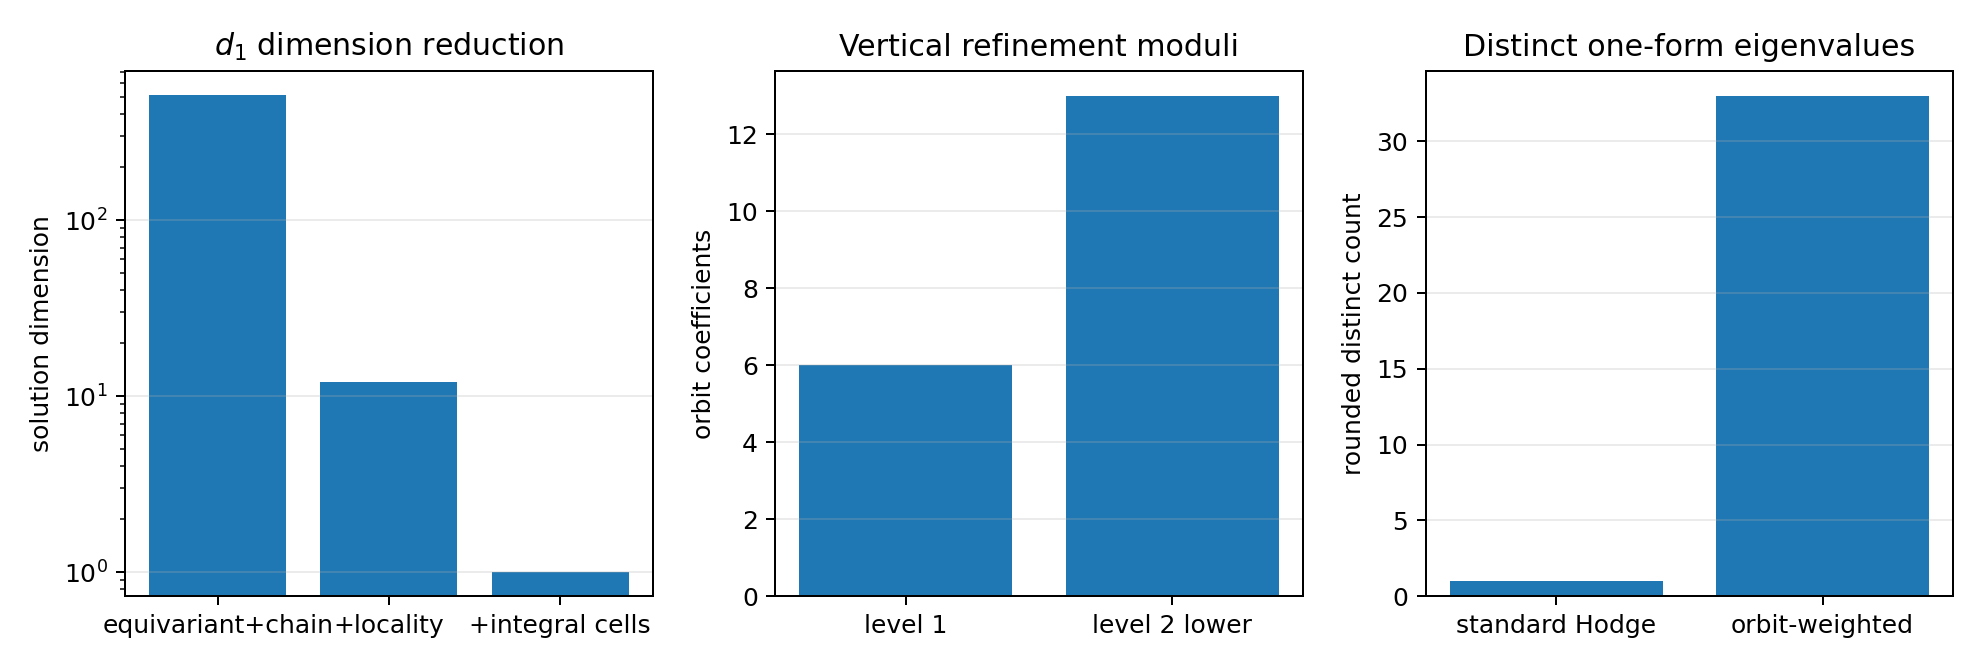
\includegraphics[width=.98\textwidth]{FIN_ST2082_ST2171_Figures/equivariant_d1_classification.png}
\caption{Left: exact dimension reduction under progressively stronger
conditions.  Centre: vertical moduli introduced by refinement.  Right: the
flat standard Hodge spectrum versus a natural orbit-weighted witness.}
\end{figure}

\section{Most important result}

The second differential itself is not the missing unique object once cellular
integrality is imposed; it becomes the standard boundary operator on whatever
cells were already chosen.  The missing information is the selection and
physical weighting of ternary/2-form structure.

Pairwise kernel data and the 0-form Dirichlet operator contain no independent
three-point observable.  Any triangle weight built afterward as a function of
three pair weights is another chosen rule, and Release 11.05 exhibited many
nonproportional natural rules.

Thus the decisive obstruction is now typed as:
\[
\boxed{
\text{strict FIN lacks an intrinsic ternary/2-form source}.}
\]

\section{Highest-value next theorem}

The new source gate requires:
\begin{enumerate}[label=T\arabic*.]
\item an intrinsic strict ternary/cycle observable;
\item a $D_{12}$ transformation law and nonzero orbit witness;
\item face-set and $d_1$ selection independent of target fitting;
\item a positive Hodge measure source;
\item $12\to24\to48$ refinement transport/coherence;
\item dimensional/continuum Maxwell scaling;
\item an $OA$ platform and record.
\end{enumerate}
The current strict repository passes zero complete rows.  Existing chiral
bispectra are valuable orientation markers but remain premise-based and do not
supply the complete face/Hodge/refinement package.

The highest-value next theorem is therefore:
\begin{quote}
\emph{derive or refute an intrinsic ternary cumulant, associator or cycle
response from the adaptive/refinement law, then test whether its orbit tensor
selects a face complex and positive Hodge measure without target fitting.}
\end{quote}

A nonzero, refinement-coherent source would introduce genuinely new information
beyond the pair kernel and could change the physical verdict.  Exhausting the
available strict ternary candidates with no passing source would be a total
no-new-live-frontier result for the gauge-geometry route.

\section{Route ranking}

\begin{longtable}{@{}p{.53\textwidth}p{.18\textwidth}p{.18\textwidth}@{}}
\toprule
Route & Rigorous-success estimate & Physics decision power \\
\midrule\endhead
strict ternary/2-form source intake & 0.55 & 1.00 \\
conditional integral product-cell gauge model & 0.90 & 0.50 \\
fine-holonomy measurement of Hodge weights & 0.40 & 0.60 \\
additional pairwise face functions & 0.05 & 0.20 \\
$OA$ frozen-channel experiment & 0.45 & 0.55 \\
\bottomrule
\end{longtable}

These are strategic judgments, not empirical probabilities.

\section{Final interpretation}

\begin{quote}
For a chosen cellular complex, FIN admits a canonical primitive second
differential and coherent conditional Hodge/gauge models.  Neither equivariance,
locality, refinement, positivity, cohomology nor spectra choose the cells and
their Hodge weights from current pairwise data.  FIN remains a finite
Dirichlet--Markov--spectral information geometry with conditional gauge
extensions, not a fundamental physical theory.  The intrinsic ternary-source
audit is the next point capable of changing that conclusion.
\end{quote}

\appendix
\section{Six-round ledger}
\begin{longtable}{@{}p{.18\textwidth}p{.35\textwidth}p{.37\textwidth}@{}}
\toprule
Range & Target & Verdict \\
\midrule\endhead
ST2082--ST2096 & equivariant $d_1$ & exact dimension 517 \\
ST2097--ST2111 & boundary locality & twelve orbit scales \\
ST2112--ST2126 & refinement & vertical coefficients persist \\
ST2127--ST2141 & positivity/Hodge & rescaling gauge and positive cone \\
ST2142--ST2156 & spectra/cohomology & flat/tunable spectrum no-go \\
ST2157--ST2171 & synthesis & intrinsic ternary-source frontier \\
\bottomrule
\end{longtable}

\section{Reproducibility}
The authoritative result sets run from
\path{FIN_ST2082_ST2096_Results.json} through
\path{FIN_ST2157_ST2171_Results.json}.  Each contains fifteen programmes and
packet SHA-256 references.  The combined test
\path{test_fin_st2082_st2171.py} verifies all ninety packets, character
dimensions, locality reduction, refinement moduli, Hodge identity, spectra,
updated gate, figure and nonpromotion boundaries.

\section{Nonclaims}
This report does not derive an intrinsic ternary source, a unique face complex,
Hodge measure, gauge coupling, continuum Maxwell theory, physical scale, state
ontology, platform or evidence.  It does not complete legacy role transfer,
QW-2191, Standard Model, gravity, $L_{\rm total}$ or Theory of Everything.  All
future FIN PDFs remain English.

\begin{thebibliography}{9}
\bibitem{serre} J.-P. Serre, \emph{Linear Representations of Finite Groups}, Springer.
\bibitem{hatcher} A. Hatcher, \emph{Algebraic Topology}, Cambridge University Press.
\bibitem{desbrun} M. Desbrun et al., Discrete Exterior Calculus, arXiv:math/0508341.
\end{thebibliography}
\end{document}
